% Options for packages loaded elsewhere
% Options for packages loaded elsewhere
\PassOptionsToPackage{unicode}{hyperref}
\PassOptionsToPackage{hyphens}{url}
\PassOptionsToPackage{dvipsnames,svgnames,x11names}{xcolor}
%
\documentclass[
  authoryear,
  preprint,
  3p]{elsarticle}
\usepackage{xcolor}
\usepackage{amsmath,amssymb}
\setcounter{secnumdepth}{5}
\usepackage{iftex}
\ifPDFTeX
  \usepackage[T1]{fontenc}
  \usepackage[utf8]{inputenc}
  \usepackage{textcomp} % provide euro and other symbols
\else % if luatex or xetex
  \usepackage{unicode-math} % this also loads fontspec
  \defaultfontfeatures{Scale=MatchLowercase}
  \defaultfontfeatures[\rmfamily]{Ligatures=TeX,Scale=1}
\fi
\usepackage{lmodern}
\ifPDFTeX\else
  % xetex/luatex font selection
\fi
% Use upquote if available, for straight quotes in verbatim environments
\IfFileExists{upquote.sty}{\usepackage{upquote}}{}
\IfFileExists{microtype.sty}{% use microtype if available
  \usepackage[]{microtype}
  \UseMicrotypeSet[protrusion]{basicmath} % disable protrusion for tt fonts
}{}
\makeatletter
\@ifundefined{KOMAClassName}{% if non-KOMA class
  \IfFileExists{parskip.sty}{%
    \usepackage{parskip}
  }{% else
    \setlength{\parindent}{0pt}
    \setlength{\parskip}{6pt plus 2pt minus 1pt}}
}{% if KOMA class
  \KOMAoptions{parskip=half}}
\makeatother
% Make \paragraph and \subparagraph free-standing
\makeatletter
\ifx\paragraph\undefined\else
  \let\oldparagraph\paragraph
  \renewcommand{\paragraph}{
    \@ifstar
      \xxxParagraphStar
      \xxxParagraphNoStar
  }
  \newcommand{\xxxParagraphStar}[1]{\oldparagraph*{#1}\mbox{}}
  \newcommand{\xxxParagraphNoStar}[1]{\oldparagraph{#1}\mbox{}}
\fi
\ifx\subparagraph\undefined\else
  \let\oldsubparagraph\subparagraph
  \renewcommand{\subparagraph}{
    \@ifstar
      \xxxSubParagraphStar
      \xxxSubParagraphNoStar
  }
  \newcommand{\xxxSubParagraphStar}[1]{\oldsubparagraph*{#1}\mbox{}}
  \newcommand{\xxxSubParagraphNoStar}[1]{\oldsubparagraph{#1}\mbox{}}
\fi
\makeatother


\usepackage{longtable,booktabs,array}
\newcounter{none} % for unnumbered tables
\usepackage{calc} % for calculating minipage widths
% Correct order of tables after \paragraph or \subparagraph
\usepackage{etoolbox}
\makeatletter
\patchcmd\longtable{\par}{\if@noskipsec\mbox{}\fi\par}{}{}
\makeatother
% Allow footnotes in longtable head/foot
\IfFileExists{footnotehyper.sty}{\usepackage{footnotehyper}}{\usepackage{footnote}}
\makesavenoteenv{longtable}
\usepackage{graphicx}
\makeatletter
\newsavebox\pandoc@box
\newcommand*\pandocbounded[1]{% scales image to fit in text height/width
  \sbox\pandoc@box{#1}%
  \Gscale@div\@tempa{\textheight}{\dimexpr\ht\pandoc@box+\dp\pandoc@box\relax}%
  \Gscale@div\@tempb{\linewidth}{\wd\pandoc@box}%
  \ifdim\@tempb\p@<\@tempa\p@\let\@tempa\@tempb\fi% select the smaller of both
  \ifdim\@tempa\p@<\p@\scalebox{\@tempa}{\usebox\pandoc@box}%
  \else\usebox{\pandoc@box}%
  \fi%
}
% Set default figure placement to htbp
\def\fps@figure{htbp}
\makeatother





\setlength{\emergencystretch}{3em} % prevent overfull lines

\providecommand{\tightlist}{%
  \setlength{\itemsep}{0pt}\setlength{\parskip}{0pt}}



 
\usepackage[]{natbib}
\bibliographystyle{elsarticle-harv}


\usepackage{booktabs}
\usepackage{longtable}
\usepackage{array}
\usepackage{multirow}
\usepackage{wrapfig}
\usepackage{float}
\usepackage{colortbl}
\usepackage{pdflscape}
\usepackage{tabularx}
\usepackage{xltabular}
\usepackage{threeparttable}
\usepackage{threeparttablex}
\usepackage[normalem]{ulem}
\usepackage{makecell}
\usepackage{xcolor}
\usepackage{tcolorbox}
\makeatletter
\@ifpackageloaded{caption}{}{\usepackage{caption}}
\AtBeginDocument{%
\ifdefined\contentsname
  \renewcommand*\contentsname{Table of contents}
\else
  \newcommand\contentsname{Table of contents}
\fi
\ifdefined\listfigurename
  \renewcommand*\listfigurename{List of Figures}
\else
  \newcommand\listfigurename{List of Figures}
\fi
\ifdefined\listtablename
  \renewcommand*\listtablename{List of Tables}
\else
  \newcommand\listtablename{List of Tables}
\fi
\ifdefined\figurename
  \renewcommand*\figurename{Figure}
\else
  \newcommand\figurename{Figure}
\fi
\ifdefined\tablename
  \renewcommand*\tablename{Table}
\else
  \newcommand\tablename{Table}
\fi
}
\@ifpackageloaded{float}{}{\usepackage{float}}
\floatstyle{ruled}
\@ifundefined{c@chapter}{\newfloat{codelisting}{h}{lop}}{\newfloat{codelisting}{h}{lop}[chapter]}
\floatname{codelisting}{Listing}
\newcommand*\listoflistings{\listof{codelisting}{List of Listings}}
\makeatother
\makeatletter
\makeatother
\makeatletter
\@ifpackageloaded{caption}{}{\usepackage{caption}}
\@ifpackageloaded{subcaption}{}{\usepackage{subcaption}}
\makeatother
\journal{International Journal of Human-Computer Studies}
\usepackage{bookmark}
\IfFileExists{xurl.sty}{\usepackage{xurl}}{} % add URL line breaks if available
\urlstyle{same}
% fallback for those not using the hyperref driver hyperxmp:
\makeatletter
\@ifundefined{xmpquote}{\newcommand{\xmpquote}[1]{#1}}{}
\makeatother
\hypersetup{
  pdftitle={Using Data Visualisation to Influence Donation Behaviour},
  pdfauthor={Gabriel Strain; Aadityaa Mehrotra; Paul A. Warren; Caroline Jay; Andrew J. Stewart},
  pdfkeywords={\xmpquote{donation
behaviour}, \xmpquote{scatterplot}, \xmpquote{crowdsourced}},
  colorlinks=true,
  linkcolor={blue},
  filecolor={Maroon},
  citecolor={Blue},
  urlcolor={Blue},
  pdfcreator={LaTeX via pandoc}}


\setlength{\parindent}{6pt}
\begin{document}

\begin{frontmatter}
\title{Using Data Visualisation to Influence Donation Behaviour}
\author[1]{Gabriel Strain%
\corref{cor1}%
}
 \ead{gabriel.strain@manchester.ac.uk} 
\author[1]{Aadityaa Mehrotra%
%
}
 \ead{aadityaa.mehrotra@student.manchester.ac.uk} 
\author[2]{Paul A. Warren%
%
}
 \ead{paul.warren@manchester.ac.uk} 
\author[1]{Caroline Jay%
%
}
 \ead{caroline.jay@manchester.ac.uk} 
\author[1]{Andrew J. Stewart%
%
}
 \ead{andrew.j.stewart@manchester.ac.uk} 

\affiliation[1]{organization={University of Manchester, Department of
Computer Science, Faculty of Science and
Engineering},addressline={Oxford Road},city={Manchester},country={United
Kingdom},countrysep={,},postcode={M13 9PL},postcodesep={}}
\affiliation[2]{organization={University of Manchester, Division of
Psychology, Communication and Human Neuroscience, School of Health
Sciences, Faculty of Biology, Medicine, and Health},addressline={Oxford
Road},city={Manchester},country={United
Kingdom},countrysep={,},postcode={M13 9PL},postcodesep={}}

\cortext[cor1]{Corresponding author}





        
\begin{abstract}
Can optimising scatterplots to support correlation perception also
influence financial decision-making? Previous research has shown that
relatively small changes in the visual design of scatterplots can affect
perceived correlation and the extent to which people update their
beliefs. Here, we test whether such perceptual effects not only impact
beliefs, but are also able to influence subsequent behaviours. In a
fully reproducible online experiment using a charitable allocation
paradigm, we show that scatterplots optimised for correlation perception
also influence behavioural outcomes, and that participants engage with
and incorporate data visualisations into their decisions and behaviours.
These findings indicate that visual design choices have practical
consequences for domains in which data visualisations are used to inform
judgement, persuasion, and decision-making. We discuss the implications
for the use of data visualisations in advertising and identify future
directions for research on behaviour change following exposure to visual
information.
\end{abstract}





\begin{keyword}
    donation behaviour \sep scatterplot \sep 
    crowdsourced
\end{keyword}
\end{frontmatter}
    

\section{Introduction}\label{sec-intro}

Can data visualisation be used to change the ways people behave? Far
from being solely used by academics and professionals, data
visualisations are now an everyday part of many people's lives. From
visualisations of health data during the COVID-19 pandemic, to those
illustrating statistics in live sports reporting, the ability of data
visualisation to scaffold understanding of numerical data has led to
widespread adoption across scientific and health communication, news
media, and policy making. Traditionally, data visualisation design has
been technician-led; designers often prefer software defaults
\citep{haber_2016, petrescu_2024}, rely on personal knowledge as opposed
to design theory \citep{parsons_2020}, and rely on oversimplified
guidance that fails to properly link design guidelines to actual human
perception and cognition \citep{patterson_2014}. The result of this
disconnect is a landscape saturated with misleading visualisations
\citep{wtf_2026}; whether due to intentional deception
\citep{pandey_2015} or a lack of understanding, it is clear that there
is a need for more work studying how we design visualisations based on
established perceptual and cognitive phenomena.

Part of designing visualisations in such a way is understanding how
small variations in them, of the kind that might traditionally be
thought of as purely aesthetic choice, can change the perceptions,
cognitions, and behaviours of those who view them. Recent work
investigating a novel form of scatterplot point encoding found that
lowering the opacity and size of scatterplot points as a function of
residual magnitude, both separately \citep{strain_2023, strain_2023a}
and together \citep{strain_2024}, can have significant effects on
perceptions of correlation. These techniques were used to correct for a
longstanding underestimation bias, and have additionally been shown to
affect the degree to which people's beliefs about the levels of
relatedness between a variable pair change \citep{strain_2025}. In
addition to providing new options to designers who wish to highlight
different visualisation features, studies such as these can provide
insight into how data concepts are interpreted more generally by
viewers.

Testing whether visualisation modifications such as these are able to
affect not only how we perceive data, but also our subsequent actions is
a much harder problem to solve. To this end, we present a single,
crowdsourced, online experiment that situates novel scatterplot
visualisation techniques in charity infographics. We use a forced
donation allocation task, whereby participants must share money between
charities represented by infographics including standard and alternative
scatterplots, and collect and analyse participants' charity preferences
and donation allocation behaviours. We build a range of models to show
that while preference for charitable concerns is responsible for most of
the variance in donation allocation behaviour, both the data displayed
in the plot and the alternative scatterplot point encoding have
significant effects.

\section{Related Work}\label{sec-related-work}

We begin this section by reviewing the literature at the intersection of
data visualisation and behaviour change. We then explore our chosen
behaviour-change paradigm, donation behaviour, particularly in response
to infographics and other forms of informative advertising. This section
concludes by reviewing the modified scatterplots used to elicit
behaviour change in the present study, followed by a statement of our
hypotheses.

\subsection{Behaviour and Data
Visualisation}\label{sec-behaviour-data-viz}

Data visualisation, broadly defined as the practice of presenting
information in a visual modality \citep{hinterberger_2009}, is widely
relied upon for the communication of simple and complex statistical and
numerical data and concepts. From infographics designed to promote
health behaviours to complex multiclass scatterplot matrices used for
exploratory data analysis in machine learning paradigms, pictorial
representations of data are ubiquitous. On a base level, their
popularity speaks to the human tendency to represent our world visually.
Despite this, there is relatively little literature exploring how data
visualisation may affect the ways people behave. Clearly, there is the
assumption (or hope), that data visualisations are able to affect
behaviour to a certain degree. If this were not the case, they would not
be displayed in hospitals to promote positive health behaviours or by
environmental charities to promote environmentally friendly choices.
There is a wealth of evidence suggesting that data visualisations in
different forms can affect perceptions of underlying data; varying the
sizes and opacities of scatterplot points can change perceptions of
correlation \citep{strain_2023, strain_2023a, strain_2024}, perceptions
of data magnitudes and ratio are affected by axis orientations and
truncation \citep{bradley_2025, mckinley_2026}, and line characteristics
affect judgements of global means in line charts \citep{moritz_2024}.

There is also a body of literature that provides evidence that
perceptual effects may influence cognition. Scatterplots featuring
points with varying opacities and sizes can affect the levels to which
viewers update their beliefs \citep{strain_2025}, risk information
presented graphically can increase stated risk-avoidant behaviour
\citep{stone_1997, schirillo_2005}, and data visualisation can be used
to improve decision-making performance
\citep{cheong_2016, padilla_2018}. Given evidence that data
visualisation can, in some contexts, be more persuasive than the
equivalent information presented in a tabular format
\citep{pandey_2014}, it remains to be seen whether perceptual and
cognitive effects of data visualisation can drive differences in
behaviour.

There is some evidence that effects such as those described above are
driven by data visualisation promoting higher levels of engagement with
the underlying data. \citet{rudolph_2009} found that the use of a visual
analytics tool was able to increase levels of task engagement and
learning, resulting in improved financial decision-making amongst
non-expert participants when compared to those presented only with
tabular data, while \citet{fu_2025} found that static and dynamic
visualisation promoted higher levels of learning motivation and
engagement with algorithm learning amongst students. In a longitudinal
study of participant-created `vernacular visualisations',
\citet{abos_2024} found that creating visualisations helped participants
develop and maintain habits that reduced food waste. This improvement
was attributed to increased engagement with the self-created
visualisation format.

Testing real behaviour change in response to visualisation viewing is
necessarily difficult; lab or online testing may fail to induce enough
of a sense of realism to extract actual behaviour, while longitudinal
testing is difficult and expensive to carry out. In the present study,
we use a deception technique to elicit participants' real behavioural
intentions, which have been shown to be a moderate predictor of actual
behaviour \citep{webb_2006, conner_2022}.

\subsection{Donation Behaviour}\label{sec-donation-behaviour}

With around 32\% of the UK charity sector's income coming from donations
and legacies \citep{gov_report}, reaching new donors and encouraging
them to give more is a key part of running a successful charity
\citep{sargeant_2001, wymer_2006}, as efficient spending on advertising
and other fundraising activities leaves more money to be spent on
charitable activities. Data visualisation, which has been shown in some
contexts to be more persuasive than textual information
\citep{pandey_2014} and able to affect the levels to which people change
their beliefs \citep{karduni_2021, markant_2023, strain_2025}, is a
relatively untapped resource with regards to creating more effective
advertising materials. Investigations of the use of anthropomorphic
visualisation have found limited evidence for their efficacy with regard
to increasing donation amounts \citep{boy_2017, morais_2021}, while
showing real pictures to potential donors (the so-called
\emph{Identifiable Victim Effect}) has been shown to have positive
effects on donation \citep{genevsky_2013}.

The literature on donation behaviour is generally focused on the
characteristics of donors, and often makes a distinction between
choosing to donate at all and the amount donated. \citet{green_1997}
used factor analysis and an interdisciplinary literature review to
identify seven factors associated with charitable giving behaviour. Five
of these were motivations for giving, and included altruism, negative
state relief, and social exchange. \citet{gittell_2006} identify
economic, religious, and demographic factors influencing giving rates,
with higher levels of personal income, protestantism, and education
positively impacting donations. More recently, \citet{neumayr_2019}
identified subjective dispositions, such as trust, empathic concern, and
religious affiliation as predictive of the decision to donate (but not
the amount); what they term \emph{human resources}, such as income and
education level, impact both the decision to donate and the amounts
people choose to give. \citet{bekkers_2011} provide a detailed review of
the person-specific mechanisms that drive charitable giving. Despite
this literature, it remains difficult to design donation-eliciting
campaigns that appeal across the range of personal characteristics that
may motivate donation behaviour.

The weight of evidence generally points towards donation decisions being
strongly influenced by personal preferences of charities and charitable
concerns, although the literature is not in full agreement. In a
qualitative study of 60 donors, \citet{breeze_2013} found that donors
are more likely to give to charities that they personally like and that
align with their values. \citet{berman_2018}, in a quantitative study
designed to increase donation amounts using principles of effective
altruism \citep{macaskill_2019}, found that participants donated more to
charities that they preferred, even when transparently more effective
options were made available to them; this was explained as being a
result of an emotional connection to the cause being valued over
rational decision making and reasoned argument. In opposition,
\citet{she_2023} found that charity preference had no effect on donation
amounts in an online dictator game-style study. The disagreement here
motivated the collection of charity preference ratings and rankings in
the present study.

\subsection{Correlation Perception and Modified
Scatterplots}\label{sec-corr-percept}

In addition to testing whether data visualisation can influence donation
allocation decisions, we also aim to test a recently developed
scatterplot visualisation technique. Scatterplots, which are primarily
used to visualise the correlation between pairs of variables, are a
widely used type of data visualisation \citep{tufte_1983}. Historically,
there has been evidence of a bias in correlation estimation in
scatterplots; positive correlation is routinely underestimated. This
finding has been replicated in direct estimation paradigms, where
participants are asked to provide a numerical estimate of correlation
\citep{strahan_1978, bobko_1979, cleveland_1982, lane_1985, lauer_1989, collyer_1990, meyer_1992},
and in those asking participants to estimate correlation via a bisection
task \citep{rensink_2017}. The underestimation is particularly
pronounced for bivariate data with Pearson's \emph{r} in the range 0.2
\textless{} \emph{r} \textless{} 0.6.

Partially inspired by evidence that estimates of means can be biased by
changing the opacities and sizes of scatterplot points
\citep{hong_2022}, recent work aiming to correct for this bias has been
successful. Strain et al.
\citetext{\citeyear{strain_2023}; \citeyear{strain_2023a}; \citeyear{strain_2024}}
systematically varied the opacities and sizes of scatterplot points to
manipulate perceptions of correlation in crowdsourced online
experiments. Using Equation 1 to relate point opacity and size to
residual magnitude, they were able to achieve significant amounts of
correction, suggesting that correlation perception may be related to
point salience.

\begin{equation}
  point_{size/opacity} = 1 - 0.25^{residual}
\end{equation}

Examples of scatterplots that use these modifications can be seen on the
top row of Figure~\ref{fig-raw-example-plots}. In addition to being able
to manipulate estimates of correlation, there is also evidence that the
same technique can change the extent to which participants update their
beliefs about the levels of relatedness between a pair of variables
\citep{strain_2025}. While the effects on perception and belief change
of scatterplot visualisation techniques such as these have been
demonstrated, it remains to be seen whether they can additionally affect
behavioural intention.

\section{Hypotheses}\label{sec-hypotheses}

Our experiment seeks to investigate the impact of alternative
scatterplot design techniques on donation behaviour. We expected any
effects found to be small relative to the effect of other factors (such
as charity preference), meaning we designed our experiment to capture
these small effects. To this end, we used a forced donation allocation
paradigm, whereby participants had to share a fixed total of \(\$100\)
between two fictional charities based on their infographics.
Participants therefore provided two linked outputs per trial which were
reduced to a donation allocation ratio between the left and right-hand
charities. We formulate the first hypothesis based on previous evidence
that people will donate more money to charitable concerns that they
prefer:

\begin{itemize}
\tightlist
\item
  H\textsubscript{1}: participants will donate more money to charities
  that they prefer, as tested by Likert scales and a charity ranking.
\end{itemize}

Owing to evidence that stronger relationships portrayed in scatterplots
can induce belief change in viewers, and that features of data
visualisations can have effects on viewers' thoughts and attitudes, we
formulate the second hypothesis:

\begin{itemize}
\tightlist
\item
  H\textsubscript{2}: participants will donate more money to charities
  whose infographics feature scatterplots with higher \emph{r} values.
\end{itemize}

Finally, in light of evidence that modified scatterplots can produce
higher estimates of correlation and greater levels of belief change
regarding relatedness, we formulate the third hypothesis. This
hypothesis is non-directional due to small effects sizes reported in a
previous study that utilised these techniques
\citep{strain_2024, strain_2025}:

\begin{itemize}
\tightlist
\item
  H\textsubscript{3}: participants' donation amounts will be affected
  (non-directionally) by the type (standard or alternative) of
  scatterplot displayed.
\end{itemize}

\section{Methodology}\label{sec-methods}

In this section we begin by discussing our research methods, including
the open and reproducible research practices we used and the modelling
paradigms utilised in our analyses. We then detail the design of our
stimuli, the design of the experiment, the experimental procedure, and
participant recruitment and characteristics.

\subsection{Open Research}\label{sec-open-research}

The experiment was conducted according the principles of open and
reproducible research \citep{ayris_2018}. Hypotheses and analysis plans
were pre-registered with the Open Science Framework (OSF)\footnote{https://osf.io/bmg5z}.
All data and analysis code are included in a GitHub
repository\footnote{https://github.com/gjpstrain/behaviour\_change\_correlation\_viz\_type},
which also contains instructions for building a Docker container
\citep{boettiger_2015} that reproduces the computational environment in
which the paper was written. By capturing package versions and
dependencies using the \texttt{renv} package \citep{ushey_2026} in R,
this container allows for full replication of all stimuli, figures,
analyses, and the paper itself. Ethical approval was granted by the
University of Manchester's Proportionate University Research Ethics
Committee (Reference: 2026-26031-46636).

\subsection{Modelling}\label{sec-modelling}

Each experimental trial featured two stimuli. As participants were asked
to split \(\$100\) between the two charities displayed in the
infographics, each trial also featured two linked responses. For
modelling purposes, each pair of linked responses was reduced to a
donation allocation ratio between the left and right infographics; a
ratio value of 1 corresponds to all money being allocated to the left
charity, while a value of 0 corresponds to all money being allocated to
the right charity. This ratio, in range \([0,1]\) exists on a beta
distribution. In its standard form, beta regression cannot handle values
of precisely 0 or 1 \citep{ferrari_2004}. \citet{smithson_2006} proposed
transforming values at the boundary of the distribution to force it into
\((0,1)\). This method has faced criticism for actively distorting the
data, so we instead chose to use Kubinec's \citeyearpar{kubinec_2022}
ordered beta regression, which allows for the building of a single model
that takes into account the continuous \((0,1)\) range and the \([0,1]\)
bounds. These models were fitted using the \texttt{glmmTMB} package
\citep[version 1.1.14,][]{mcgillycuddy_2025}. All models featured random
intercepts for both participants and experimental items.

\subsection{Stimuli}\label{sec-stimuli}

\subsubsection{Charities}\label{sec-stimuli-charities}

Three charitable concerns were chosen for the experiment. Initially, we
intended to use the five charitable concerns provided in
\citet{she_2023}. These were:

\begin{enumerate}
\def\labelenumi{\arabic{enumi}.}
\tightlist
\item
  Dog Rescue and Re-housing.
\item
  Environmental Protection.
\item
  Mental Health Helpline.
\item
  Education in Disadvantaged Communities.
\item
  Support for Homeless Individuals.
\end{enumerate}

Due to our inclusion of different correlations and scatterplot types,
the use of five charity categories would have resulted in an unfeasibly
large number of experimental trials. Concerns about participant fatigue
and experimental length led us to use only the first three charity
categories for the present experiment. After deciding on the three
charity categories, one author created candidate fictional charities for
each. Two authors then decided on a single fictional charity for each
category. Table \ref{tbl-candidate-charities} shows the candidate
charities for each charity category. The final chosen charity is
highlighted in each case.

\begin{table*}

\caption{\label{tab:unnamed-chunk-1}\label{tbl-candidate-charities}The three chosen charity categories, along with the candidate fictional charities for each. The final chosen charity for each category is marked in bold and with an asterisk in each case.}
\centering
\begin{tabular}[t]{lll}
\toprule
Dog Rescue \& Re-housing & Environmental Protection & Mental Health Helpline\\
\midrule
West England Dog Re-Homing Centre & Welsh River Cleanup & SpeakUp\\
\textbf{Great British Dog Foundation*} & \textbf{Action for a Greener World*} & \textbf{Good Samaritans*}\\
London Dog’s Trust & British Bird’s Trust & Listen UK\\
\bottomrule
\end{tabular}
\end{table*}

\subsubsection{Charity Templates}\label{sec-stimuli-charity-templates}

For each of the three selected charities, we developed a corresponding
infographic to be presented during the experimental trials. These
infographics were designed to appear realistic and included fictional
charity-specific details, such as taglines, email addresses, website
links, physical addresses, and impact metrics (e.g., ``5000 + Dog Lives
Impacted''). In addition, the infographics contained secondary
background graphics that corresponded to the theme of the charity being
represented. Each charity template was designed by a single author using
Canva (www.canva.com) and checked by co-authors. Each template featured
a blank central space into which the scatterplot visualisations (see
Figure~\ref{fig-raw-example-plots}) were later inserted. Figure
\ref{fig-templates} shows the charity templates used. Each infographic
featured a scatterplot visualisation positioned centrally, which served
as the primary visual element and the main focus of the experimental
stimulus.

\begin{figure*}
  \centering
    \begin{subfigure}[t]{0.3\textwidth}
      
\includegraphics[width=\linewidth]{dog_rescue.png}
      \caption{Dog Rescue and Re-housing Charity.}
    \end{subfigure}
\hfill
    \begin{subfigure}[t]{0.3\textwidth}
      
\includegraphics[width=\linewidth]{greener_world.png}
      \caption{Environmental Protection Charity.}
    \end{subfigure}
\hfill
    \begin{subfigure}[t]{0.3\textwidth}
      
\includegraphics[width=\linewidth]{samaritans.png}
      \caption{Mental Health Helpline Charity.}
    \end{subfigure}
  \caption{Charity templates based on the three selected fictional charities.}
  \label{fig-templates}
\end{figure*}

\subsubsection{Scatterplot
Visualisations}\label{sec-stimuli-visualisations}

Previous work has shown that changes to the opacities and sizes of
scatterplot points can induce changes in perceptions of correlation in
viewers \citep{strain_2023, strain_2023a, strain_2024}. In particular,
lowering the opacity and size of points as a function of residual
magnitude is able to bias estimates of correlation upwards and partially
correct for an observed underestimation bias in positively correlated
scatterplots. The same techniques have also been shown to be able to
induce greater levels of belief change in viewers of scatterplots
contextualised as part of news items \citep{strain_2025} when compared
to traditional plots. To test whether such effects can be extended to
change behaviours, we use the same technique here. In the alternative
scatterplot condition, point opacity and size is reduced as a function
of residual magnitude using Equation 1. To facilitate comparison to
previous work also examining alternatively designed scatterplots
\citep{strain_2023, strain_2023a, strain_2024, strain_2025}, we elect to
use the same scatterplot generation protocol in the present study. This
includes the number of scatterplot points (n = 128), and the size
scaling factor and opacity floor used to increase point visibility. We
chose to use three Pearson's \emph{r} values: 0.2, 0.5, and 0.8. If
participants are engaging with the visualisations and using them to
inform their donation decisions, then plots featuring higher \emph{r}
values should attract greater proportions of donated money. If the
effects on perception and belief change seen previously with
scatterplots of the type featured in the alternative condition can be
extended to change behaviour, then alternative scatterplots should
elicit greater donations.

Each scatterplot was positively correlated, and featured identical
\(x\)-axis labels regarding donation amount. Each charity's \(y\)-axis
label related to a realistic outcome variable for the particular charity
category featured. Examples of standard and alternative scatterplots for
each \emph{r} value used can be seen in
Figure~\ref{fig-raw-example-plots}, while full charity template +
scatterplot visualisation examples can be seen as part of Figure
\ref{fig-example-trial}.

\begin{figure*}

\centering{

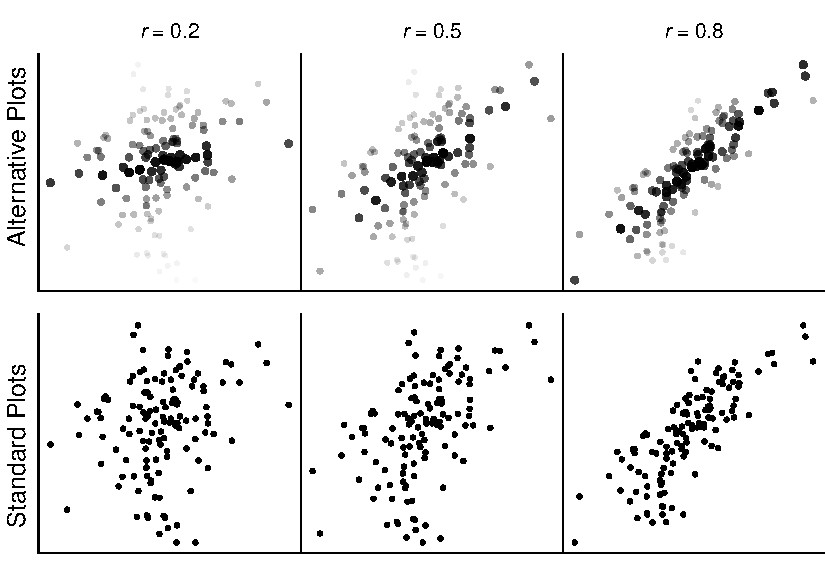
\includegraphics[width=1\linewidth,height=\textheight,keepaspectratio]{fig-raw-example-plots-1.pdf}

}

\caption{\label{fig-raw-example-plots}Scatterplots for each of the three
\textit{r} values. Separate rows are provided for the alternative (top)
and standard (bottom) conditions. The data are identical in each column.
Only the sizes and opacities of points are altered in the top row.}

\end{figure*}%

\subsection{Design}\label{sec-design}

We employed a fully within-subjects design. With 18 unique plots (3
charities \(\times\) 3 correlation values \(\times\) 2 plot types), all
unique combinations would result in \(\binom{18}{2} = 153\) pairs. To
decrease the task load on participants, we removed the 45 trials which
featured the same charity for a final total of 108 experimental trials.
Participants viewed all 108 experimental trials, along with 6 attention
check trials, in a fully randomised order. Our dependent variable was
the amount of money participants assigned to the left and right charity
infographics on a per-trial basis, collapsed into a single ratio value.
The experiment, including all stimuli, materials, and instructions, is
hosted on GitLab\footnote{https://pavlovia.org/Strain/donation\_behaviour}.

\subsection{Procedure}\label{sec-procedure}

The experiment was built using PsychoPy \citep{peirce_2019} and is
hosted on Pavlovia.org. Participants were instructed to only complete
the experiment on desktop or laptop computers. Each participant first
viewed the participant information sheet and provided consent by
checking boxes next to consent statements. Consent was required in order
to progress through the experiment. They were asked to provide their age
in a free-text box, followed by their gender identity. Using Likert
scales, participants were then asked to indicate how important the three
chosen charitable concerns were to them (Dog Rescue and Re-Housing,
Environmental Protection, and Mental Health Helpline). Each Likert scale
featured seven points, and was anchored at points 1 and 7 with ``Not at
all important'' and ``Extremely important'' labels. Participants then
used a drag-and-drop interface to rank the three charitable concerns.
Following the pre-experimental tests, participants were then asked to
complete eight rounds of the Remote Associates Test (RAT), which acted
as a filler task to prevent carryover effects \citep{she_2023}.
Participants were given 15 seconds for each round of the RAT, and were
not required to answer. Participants were given instructions, including
the following:

\hspace{0pt}
\begin{tcolorbox}[colback=gray!10, colframe=gray!50, boxrule=0.5pt]
...
\newline
  5. We encourage you to make assignments as if it were your own money.
  \newline
  6. To help you get into this mindset, the research team have decided to donate money to real-life charities based on the totals donated by all participants over the course of the experiment.
  \newline
  7. Once the experiment has concluded, you will receive an email detailing how the research team have split the money and which charities have been donated to.
  \newline
  ...
\end{tcolorbox}
\hspace{0pt}

Participants were informed that this was a deception following
conclusion of the experiment. Following instructions, the experiment
began. In a series of 108 experimental trials, participants were asked
to split \(\$100\) between two charity infographics. Presentation order
was randomised, including 6 attention check trials which explicitly
asked participants to assign \(\$100\) to either the left (n = 3) or the
right (n = 3) charity infographic. An example of an experimental trial
can be seen in Figure~\ref{fig-example-trial}. After completing all
trials, participants were debriefed regarding the deception employed and
thanked for their participation.

\begin{figure*}

\centering{

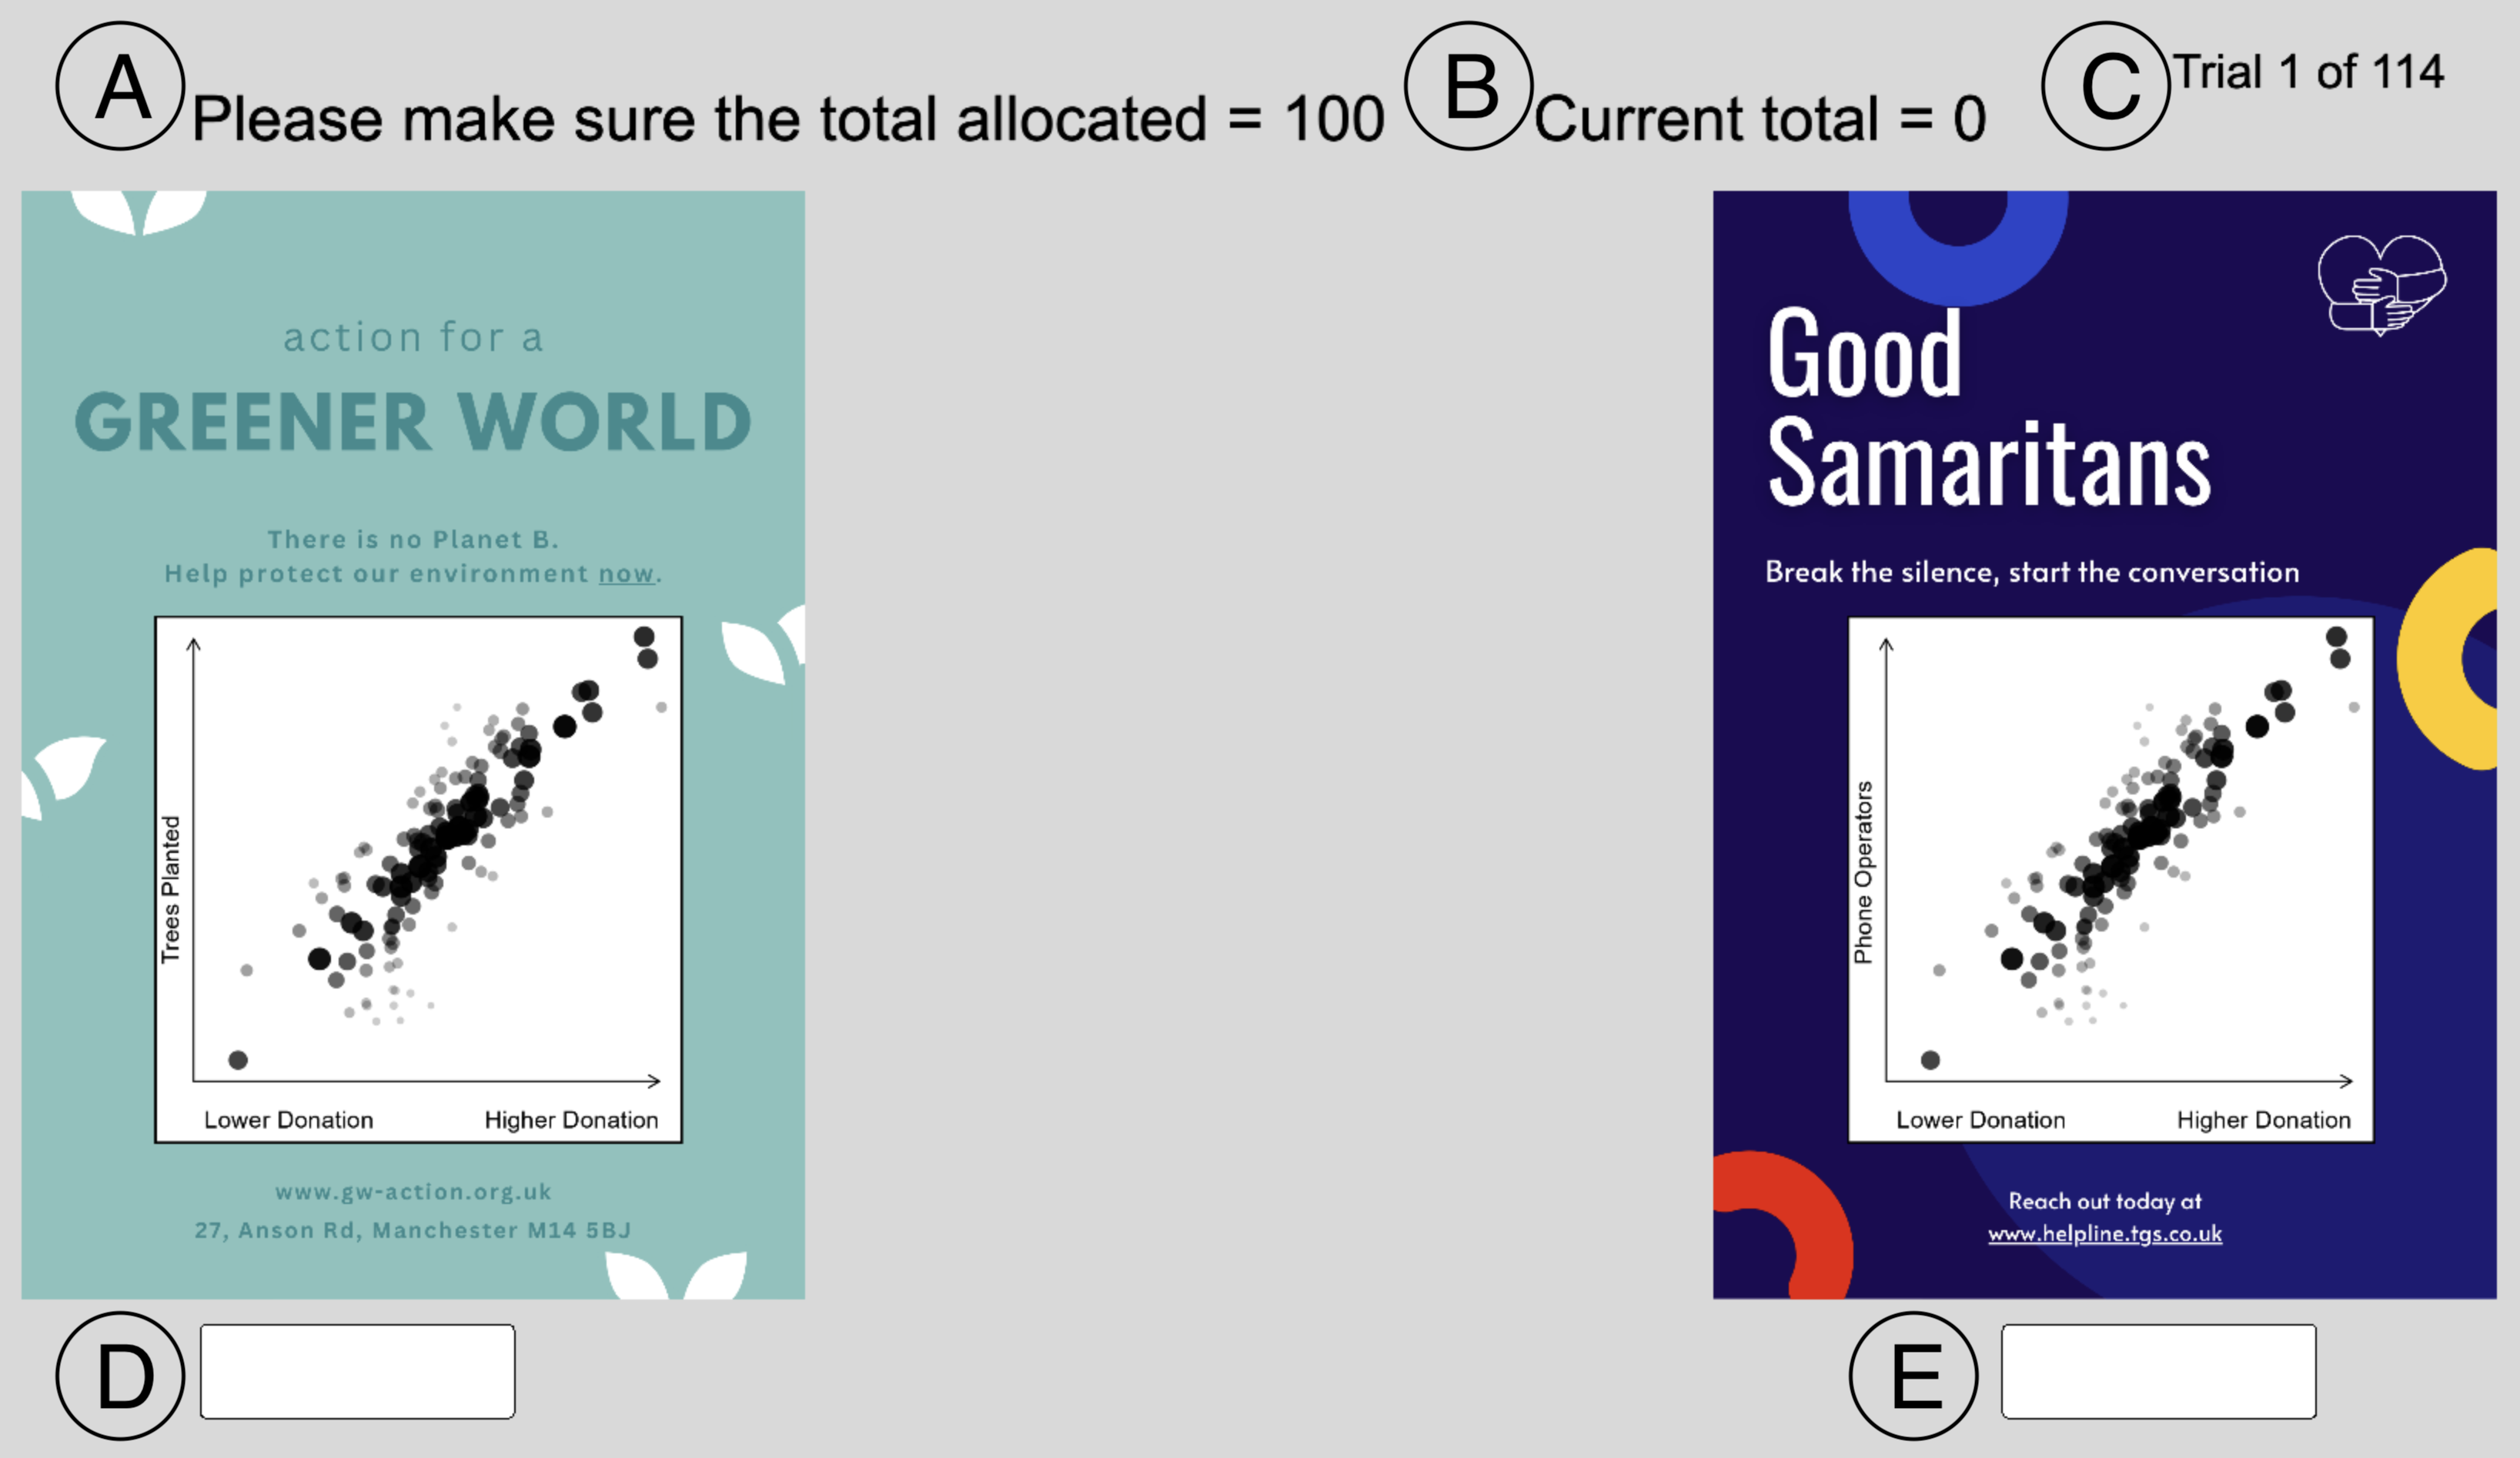
\includegraphics[width=1\linewidth,height=\textheight,keepaspectratio]{example_trial.png}

}

\caption{\label{fig-example-trial}An example of an experimental trial.
Illustrated are the reminder to use all available money (A), the display
of the current total (B), the trial counter (C), the left infographic
and allocation box (D), and the right infographic and allocation box
(E).}

\end{figure*}%

\subsection{Participants}\label{sec-participants}

Participants were recruited using \citet{prolific}. English fluency and
normal or corrected-to-normal vision were required, as well as having
not previously taken part in any of the research team's previous studies
into scatterplot visualisations
\citep{strain_2023, strain_2023a, strain_2024, strain_2025}. In an
effort to improve data quality, strict pre-screening criteria were also
employed \citep{peer_2021}; participants were required to have
previously completed at least 100 studies on the platform, and were
required to have been accepted on at least 99\% of them. Data were
collected from 174 participants. 10 failed more than 3 out of 6
attention checks, meaning their submissions were rejected in accordance
with our pre-registration\footnote{The pre-registration states that 150
  participants would be recruited. Additional participants were
  recruited due to an oversight before the data were inspected, and for
  full transparency all analyses are done using the full dataset.}. Data
from the remaining 164 participants were included in the full analysis
(86 male, 76 female, and 2 non-binary). Participants' mean age was 34.7
years (SD = 11.2 years). Participants took a mean of 25.7 minutes to
complete the experiment (SD = 7.5 minutes).

\section{Results}\label{sec-results}

All analyses were conducted using R \citep[version 4.5.3,][]{r_core}.
Each hypothesis is first tested using a model that only includes the
fixed effect of interest. A full interaction model is then fitted taking
into account all fixed effects and the potential interactions between
them. This model provides more conservative estimates; we therefore use
the \texttt{marginaleffects} package \citep[version
1.0.0,][]{arel-bundock_2024} with this model to calculate marginal
effects over the full ranges of each fixed effect in Table
\ref{tbl-marginal-effects-interactions}. All modelling uses a collapsed
per-trial ratio of left to right donation amounts. To increase
interpretability, however, descriptive statistics, including relevant
tables and visualisations, use uncollapsed donation allocation means.
All hypotheses received support and each is provided below prior to the
reporting of relevant results.

\definecolor{nicegreen}{HTML}{3EB489}

\hspace{0pt}
\begin{tcolorbox}[colback=nicegreen, colframe=gray!50, boxrule=0.5pt]
  H\textsubscript{1}: participants will donate more money to charities that they prefer, as tested by Likert scales and a charity ranking.
\end{tcolorbox}
\hspace{0pt}

To test the first hypothesis, that participants will donate greater
proportions of money to charities that they prefer, we built a pair of
models whereby the ratio of donations is predicted by the differences in
Likert ratings of charities and their ranks. With regards to the Likert
ratings, the experimental model explained significantly more variance
than the null (\(\chi^2\)(1) = 4,847.57, \emph{p} \textless{} .001),
driven by the fixed effect of Likert rating.
Figure~\ref{fig-donation-lines-1} illustrates how mean donation amounts
change over the full range of Likert responses.

With regards to charity rankings, the experimental model also explained
significantly more variance than the null (\(\chi^2\)(1) = 3,547.23,
\emph{p} \textless{} .001), driven by the fixed effect of charity rank.
Figure~\ref{fig-donation-lines-2} illustrates how mean donation amounts
change over the three charity rankings.

\begin{figure*}

\begin{minipage}[t]{0.50\linewidth}

\centering{

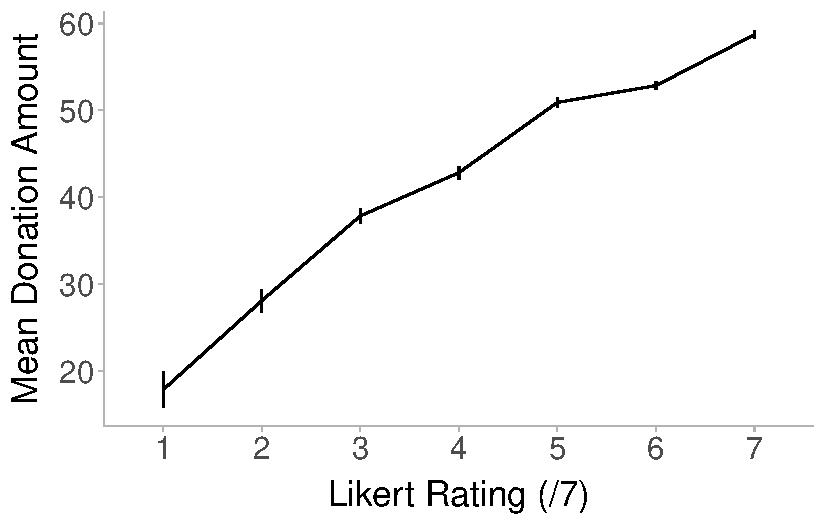
\includegraphics[width=1\linewidth,height=\textheight,keepaspectratio]{fig-donation-lines-1.pdf}

}

\subcaption{\label{fig-donation-lines-1}Mean donation allocation amounts
plotted by Likert ratings.}

\end{minipage}%
%
\begin{minipage}[t]{0.50\linewidth}

\centering{

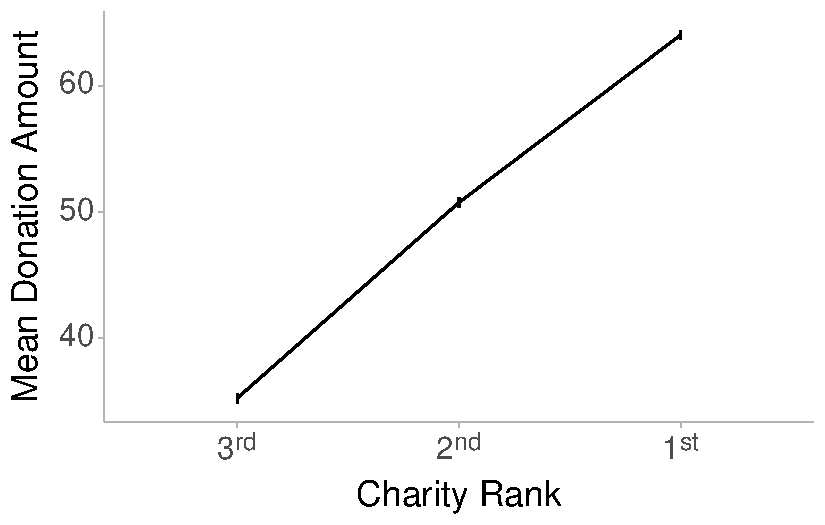
\includegraphics[width=1\linewidth,height=\textheight,keepaspectratio]{fig-donation-lines-2.pdf}

}

\subcaption{\label{fig-donation-lines-2}Mean donation allocation amounts
plotted by charity rank.}

\end{minipage}%

\caption{\label{fig-donation-lines}Mean donation allocation amounts
plotted by (a) Likert ratings, averaged across each charity rank, and
(b) charity rank, averaged across all Likert ratings. 95\% Confidence
Intervals are included as error bars. In line with H\textsubscript{1},
donation amounts increase with participants' ratings of charity
importance and as participants rank charities more highly.}

\end{figure*}%

\definecolor{nicegreen}{HTML}{3EB489}

\hspace{0pt}
\begin{tcolorbox}[colback=nicegreen, colframe=gray!50, boxrule=0.5pt]
  H\textsubscript{2}: participants will donate more money to charities whose infographics feature scatterplots with higher \textit{r} values.
\end{tcolorbox}
\hspace{0pt}

To investigate the second hypothesis, that participants will donate more
money to charity infographics that feature scatterplots with higher
\emph{r} values, we built a model where the donation ratio is predicted
by the difference in \emph{r} value between the two infographics in each
trial. The experimental model explained significantly more variance when
compared to a null model without the fixed effect of \emph{r} value
(\(\chi^2\)(1) = 119.92, \emph{p} \textless{} .001), driven by the
significant main effect of \emph{r} value. Table~\ref{tbl-donation-by-r}
shows means and standard deviations of donation amounts for each of the
three \emph{r} values used.

\begin{table}

\caption{\label{tbl-donation-by-r}Means and standard deviations of
donation allocation amounts for each \textit{r} value used.}

\centering{

\centering
\begin{tabular}{lrr}
\toprule
\multicolumn{1}{c}{Correlation Value} & \multicolumn{2}{c}{Donation} \\
\cmidrule(l{3pt}r{3pt}){1-1} \cmidrule(l{3pt}r{3pt}){2-3}
 & Mean & SD\\
\midrule
0.2 & 48.1 & 25.0\\
0.5 & 50.3 & 25.0\\
0.8 & 51.7 & 25.2\\
\bottomrule
\end{tabular}

}

\end{table}%

\definecolor{nicegreen}{HTML}{3EB489}

\hspace{0pt}
\begin{tcolorbox}[colback=nicegreen, colframe=gray!50, boxrule=0.5pt]
  H\textsubscript{3}: participants' donation amounts will be affected (non-directionally) by the type (standard or alternative) of scatterplot displayed.
\end{tcolorbox}
\hspace{0pt}

Finally, to investigate the third hypothesis, that participants'
donation allocation amounts would be affected by the type of scatterplot
used in the infographics (standard or alternative), we built a model
where donation ratio is predicted by the type of plot used. The
experimental model explained significantly more variance when compared
to a null model without the fixed effect of plot type (\(\chi^2\)(1) =
14.47, \emph{p} \textless{} .001).
Table~\ref{tbl-descriptives-donation-by-plot-type} shows means and
standard deviations of donation amounts for the two plot types, with
participants donating significantly more to charities represented by
infographics that used alternative scatterplots. Despite only explaining
a small amount of the variance in donations, this finding has
significant implications for the design of data visualisations that are
designed to drive behaviour change.

\begin{table}

\caption{\label{tbl-descriptives-donation-by-plot-type}Means and
standard deviations of donation allocation amounts for standard and
alternative plot types.}

\centering{

\centering
\begin{tabular}{lrr}
\toprule
\multicolumn{1}{c}{Plot Type} & \multicolumn{2}{c}{Donation} \\
\cmidrule(l{3pt}r{3pt}){1-1} \cmidrule(l{3pt}r{3pt}){2-3}
 & Mean & SD\\
\midrule
Standard & 49.2 & 25.0\\
Alternative & 50.8 & 25.3\\
\bottomrule
\end{tabular}

}

\end{table}%

The effects of participants' charity preference, as measured by the
Likert rating and charity ranking, are much more influential than those
of correlation value or plot type. Both to explore this more fully and
to investigate any potential interactions between our fixed effects, we
build a model where donation ratio is predicted by all four independent
variables simultaneously. This model explains significantly more
variance than a null model with no fixed effects (\(\chi^2\)(15) =
5,329.70, \emph{p} \textless{} .001). The only significant interaction
found by this model is that between charity rank and Likert ratings
(\(\chi^2(1) = 82.94\), \(p < .001\)). Given that we anticipate more
highly ranked charities to be awarded higher Likert ratings, this is an
expected finding, however we explore the interaction further in
Figure~\ref{fig-likert-rank-interactions}.

\begin{figure*}

\centering{

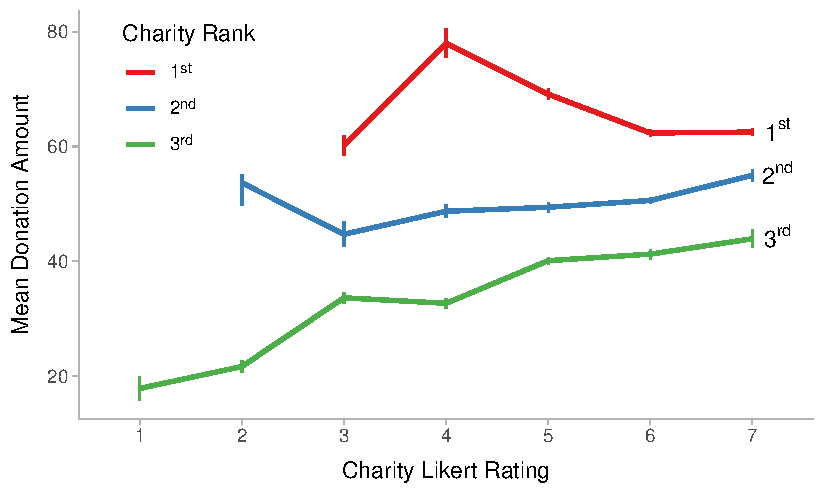
\includegraphics[width=1\linewidth,height=\textheight,keepaspectratio]{fig-likert-rank-interactions-1.pdf}

}

\caption{\label{fig-likert-rank-interactions}Mean donation amounts
plotted for each charity rank and Likert rating. Error bars show 95\%
Confidence Intervals. Note the peak in donation amount at charity rank 1
\(\times\) Likert rating 4.}

\end{figure*}%

\begin{table*}

\caption{\label{tab:unnamed-chunk-2}\label{tbl-marginal-effects-interactions}Average predicted differences in the share allocated to the left-hand charity in percentage points (pp), over the full theoretical range of each predictor. These are: Likert rating, $-6$ to $+6$; rank position, $-2$ to $+2$; correlation, $-0.6$ to $+0.6$; and plot type, $-1$ to $+1$.}
\centering
\begin{tabular}[t]{lrrrll}
\toprule
Parameter & $\Delta$ allocation (pp) & SE & $z$ & $p$ & 95\% CI\\
\midrule
Relative Likert Rating & 64.8 & 1.2 & 55.08 & <0.001 & {}[62.5, 67.1]\\
Relative Rank Position & 10.0 & 0.7 & 14.78 & <0.001 & {}[8.7, 11.4]\\
Relative Correlation & 8.0 & 0.6 & 12.51 & <0.001 & {}[6.8, 9.3]\\
Relative Plot Type & 2.8 & 0.5 & 5.40 & <0.001 & {}[1.8, 3.9]\\
\bottomrule
\end{tabular}
\end{table*}

\section{Discussion}\label{sec-discussions}

All three hypotheses were supported in this experiment. Participants'
donation allocation decisions were significantly affected by their
subjective views of the importance of the charitable concerns, by the
correlation displayed in each infographic, and by the type of
scatterplot employed. These results add to evidence that preference is
the strongest predictor of donation
\citep{breeze_2013, berman_2018, macaskill_2019}, and the finding that
higher \emph{r} values in plots increased donation amounts suggests that
participants engaged with and used the data visualisations when making
their decisions. Not only are data visualisations incorporated into
donation decisions, visual features which have previously been shown to
affect correlation estimates and belief updating (point opacity and
size) are also able to alter donation allocation behaviour. Despite only
being responsible for a small amount of donation behaviour change (see
Table \ref{tbl-marginal-effects-interactions}), the huge amounts
involved in charitable donations \citep{gov_report} mean that these
findings represent an opportunity to significantly increase donation
amounts without having to tailor the design of advertising campaigns to
different demographic groups. As this experiment represents a
behavioural proxy, further work would be required to more fully explore
the relationship between data visualisation and donation behaviour with
a view to full implementation.

\subsection{Donation Behaviour and Charity
Preferences}\label{donation-behaviour-and-charity-preferences}

In line with some previous work \citep{breeze_2013, berman_2018},
participants allocated a significantly greater proportion of money to
charities that they preferred, as measured by Likert scales and a
charity rank (see Figure~\ref{fig-donation-lines}). This finding is in
opposition to that of \citet{she_2023}, from whom the charity
categories, Likert rating, and ranking were taken. In their study,
participants were asked to play a binary choice dictator game in which
they could also assign money to themselves. As our primary interest is
in the effects of data visualisations on behaviour, we elected not to
recreate this measure, which could explain the differences in findings
between the two studies.

Figure~\ref{fig-donation-lines-1} and Figure~\ref{fig-donation-lines-2}
show the mostly linear positive relationships between donation amounts
and Likert scale ratings and charity rankings respectively. The model,
however, reveals an interaction which is visualised in
Figure~\ref{fig-likert-rank-interactions}. Visual inspection of
Figure~\ref{fig-likert-rank-interactions} suggests two possible sources
for this interaction: (1) the clear peak at Likert rating 4 that is seen
only for the 1\textsuperscript{st} charity rank, or (2) the vertical
separation between trend lines for ranks 1, 2, and 3. When participants
ranked a particular charity 1\textsuperscript{st}, their donation amount
is maximal when their Likert rating is at the midpoint of the scale.
When a charity is ranked 2\textsuperscript{nd} or 3\textsuperscript{rd}
however, the relationship between donation amount and Likert scale
rating is more linear. The mean donation amounts in
Figure~\ref{fig-likert-rank-interactions} do not take into account the
number of donation decisions for each combination of Likert scale rating
and charity rank, meaning that a very small number of high-value
donations associated with Likert rating 4 \(\times\)
1\textsuperscript{st} charity rank may have skewed the descriptive
statistics. Examining the distributions of donation decisions separately
for each charity rank and Likert scale rating in
Figure~\ref{fig-donation-histos} illustrates this. When a charity is
ranked 2\textsuperscript{nd} or 3\textsuperscript{rd}, the distribution
of donation decisions approaches normal, albeit with different central
tendencies. However, when a charity is ranked 1\textsuperscript{st}, the
distribution climbs to a peak at the top rating on the Likert scale. The
peak at Likert rating 4 \(\times\) 1\textsuperscript{st} charity rank is
actually driven by a very small number of high-value donation responses,
meaning the interaction is most likely driven by the vertical distance
between the trend lines.

\begin{figure*}

\centering{

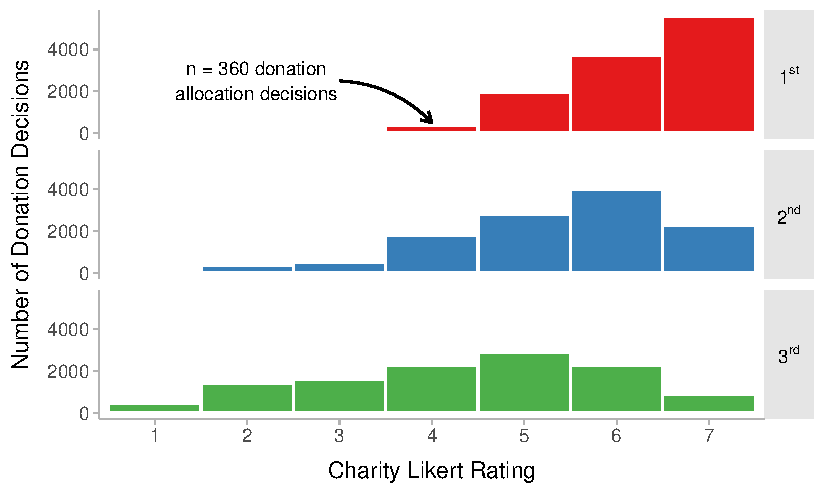
\includegraphics[width=1\linewidth,height=\textheight,keepaspectratio]{fig-donation-histos-1.pdf}

}

\caption{\label{fig-donation-histos}Donation allocation decision counts
for each charity rank and Likert rating. Note the distributions in each
case, including the very small number of donation decisions for the
charity rank 1 \(\times\) Likert rating 4 combination.}

\end{figure*}%

\subsection{Effects of Visualisations on
Behaviour}\label{effects-of-visualisations-on-behaviour}

\begin{table}

\caption{\label{tbl-RT-by-trial}Mean reaction times (RT) for trials
featuring two different scatterplots, two alternative scatterplots, and
two standard scatterplots.}

\centering{

\begin{tabular}[t]{lrr}
\toprule
Trial Type & Mean RT (s) & SD\\
\midrule
Different Plot Types & 7.69 & 4.74\\
Both Alternative & 7.46 & 4.56\\
Both Standard & 7.41 & 4.56\\
\bottomrule
\end{tabular}

}

\end{table}%

As predicted, participants donated more money to charities that featured
scatterplots with higher \emph{r} values. If participants had paid no
attention to the data visualisations present, and relied only on their
pre-existing attitudes about the charitable concerns contained in the
visualisations, then we would not expect to see a difference in
donations between scatterplots with different \emph{r} values. The
finding that lay participants engage with and utilise data
visualisations presented to them as part of a decision making and
behavioural process is a major contribution of this work. That donations
vary significantly between \emph{r} values (see
Table~\ref{tbl-donation-by-r}) suggests that the data visualisations
were being utilised by participants when they were making their donation
decisions.

As in previous work examining the effects of alternative scatterplot
design on belief updating \citep{strain_2025}, we found significant
differences in donation amounts between standard and alternative
scatterplots. Again, this finding suggests that visual features in
scatterplots are integrated into participants' donation decisions.
Examining the mean reaction times for different types of trial in
Table~\ref{tbl-RT-by-trial}, we can see that reaction times are
consistent across trial types, including when two alternative
scatterplots were presented, when two standard scatterplots were
presented, and when two different types of scatterplot were presented.
While we cannot say for certain that participants' processing of stimuli
was identical, with regards to a dual-processing account
\citep{padilla_2018}, similar reaction times suggest that the stimuli
are being processed in similar ways by participants. Evidence that
correlation is perceived rapidly by viewers of scatterplots
\citep{rensink_2014} suggests that, in the case of the present
experiment, participants were spending more time to make a more informed
decision, yet were still significantly influenced by both the \emph{r}
value of the plot in question and the specific point opacity and size
encodings utilised.

\subsection{Implications for the Design of Effective Advertising
Campaigns}\label{implications-for-the-design-of-effective-advertising-campaigns}

Previous work highlights the myriad attributes which may predict
people's donations to charitable causes
\citep{neumayr_2019, bekkers_2011, breeze_2013, berman_2018, macaskill_2019},
and the results of the present study show that most variation in
donations can be accounted for by preference for or against particular
charitable concerns. Targeted advertising \citep{iyer_2005} is able to
address some of these concerns, but necessarily requires a greater
financial investment and higher workloads -- outlays a charity may not
be able to afford. The work presented here suggests that small changes
in visual features are able to cause small changes in donation amounts.
Extrapolated out to the £27.43 billion in income derived from donations
and legacies that UK charities received in 2024 \citep{gov_report},
these small changes in donations could potentially result in large
amounts of increased income for no additional outlay.

\subsection{Limitations}\label{limitations}

The main limitation of the present study lies in whether or not
participants acted as they would when choosing where to donate their own
money. While we made efforts to lead participants to believe that their
choices in the experiment would have real-world consequences (see
Section \ref{sec-procedure}), it is impossible to know whether our
findings would be replicated in a real-world donation scenario. Reaction
times to different combinations of stimuli suggest that participants
processed both the standard and alternative scatterplots similarly;
regardless, the alternative scatterplots may have elicited distrust or
confusion in participants given their novel design. Our outcome, the
proportion of money allocated to each charity on a per-trial basis, also
limits the extent to which we can comment on real-life donation
scenarios.

\subsection{Future Work}\label{sec-future-work}

Before techniques such as those described in the present study can be
used in the real world, future work must determine whether they are able
to cause the same effects in a naturalistic setting. Testing this would
require collaboration with an organisation seeking donations, such as a
charity, and the implementation of an Online Controlled Experiment, such
as a form of A/B testing \citep{kohavi_2023}. In such a scenario,
donation amounts would be monitored while visitors to a website would be
randomly presented with either standard or alternative scatterplots. Due
to the difficulty in linking donations to advertisement/visualisation
viewing, such a study would have to take place longitudinally.

Due to the relative novelty of testing visualisations such as those
described in this study, we elected to maintain congruence between the
visualisations and the messaging in the infographics. Future work may
wish to test to what extent the effect of visualisation persists when
text-based messaging is in opposition to it. Finally, future work should
explore people's thoughts and feelings about alternative visualisation
types. There is no reason for this to be restricted to alternatively
designed scatterplots, and there is a wide range of data visualisations
that would be unfamiliar to the majority of laypeople. It may be that
any advantages of unfamiliar visualisations are outweighed by feelings
of distrust in them.

\section{Conclusion}\label{sec-conclusion}

In a fully reproducible experiment, we investigated the effects of
alternative scatterplot design on the propensity to donate money in an
online donation experiment. We collected a range of donation-relevant
participant characteristics, and showed that while charity preference
was able to explain most of the variation in donation amounts, the
statistics communicated in scatterplots (correlation) and the visual
character of those scatterplots were able to explain small but
meaningful amounts of variance. Our results suggest that alternative
scatterplot encodings which have previously been shown to influence
correlation perception and belief-updating can also have effects on
financial choices, and should be further studied as a low-cost way of
influencing behaviour.

\section*{CRediT authorship contribution
statement}\label{credit-authorship-contribution-statement}
\addcontentsline{toc}{section}{CRediT authorship contribution statement}

Gabriel Strain: Conceptualization, Data curation, Formal analysis,
Investigation, Methodology, Project administration, Resources, Software,
Visualization, Writing - Original Draft, Writing - Review \& Editing;
Aadityaa Mehrotra: Conceptualization, Resources, Writing - Review \&
Editing; Paul A. Warren: Conceptualization, Supervision, Writing -
Review \& Editing; Caroline Jay: Conceptualization, Supervision, Writing
- Review \& Editing; Andrew J. Stewart: Conceptualization, Supervision,
Validation, Writing - Review \& Editing.

\section*{Declaration of generative AI and AI-assisted technologies in
the manuscript preparation
process.}\label{declaration-of-generative-ai-and-ai-assisted-technologies-in-the-manuscript-preparation-process.}
\addcontentsline{toc}{section}{Declaration of generative AI and
AI-assisted technologies in the manuscript preparation process.}

During the preparation of this work the authors used Claude and
Microsoft Copilot to debug analysis code. After using this tool/service,
the authors reviewed and edited the content as needed and take full
responsibility for the content of the published article.

\section*{Acknowledgements}\label{acknowledgements}
\addcontentsline{toc}{section}{Acknowledgements}

This research did not receive any specific grant from funding agencies
in the public, commercial, or not-for-profit sectors.


\renewcommand\refname{References}
\bibliography{donation_behaviour.bib}



\end{document}
